\section{Experiments}
\label{sec:exp}
Every number below is generated from the released result files by the table script in the repository; numbers that run 2 has not yet produced appear as red placeholders.

\subsection{Benchmark 1: blind latent prediction}
\label{sec:pred}
\begin{table*}[t]
  \centering\small
  \caption{\textbf{Blind latent prediction} (mean over horizons 1 to 8 in the 8:16 window; MSE in whitened PCA-256
  space, mean\pm sd over seeds). Lower MSE and higher cosine are better. Every student beats both trivial predictors.
  The GRU wins; the connectome beats every sparse control and the dense net on NYC but not the dense net on the arena.}
  \label{tab:pred}
  \resizebox{\linewidth}{!}{\begin{tabular}{lcccccc}
    \toprule
    & \multicolumn{2}{c}{Arena (5 seeds)} & \multicolumn{2}{c}{Cont.\ turns (0 seeds)} & \multicolumn{2}{c}{NYC twin (3 seeds)} \\
    \cmidrule(lr){2-3}\cmidrule(lr){4-5}\cmidrule(lr){6-7}
    wiring & MSE $\downarrow$ & cos $\uparrow$ & MSE $\downarrow$ & cos $\uparrow$ & MSE $\downarrow$ & cos $\uparrow$ \\
    \midrule
    GRU, parameter-matched & \textbf{0.434\pm0.004} & \textbf{0.72} & -- & -- & \textbf{0.609\pm0.003} & \textbf{0.56} \\
    GRU, recurrent-budget-matched & 0.501\pm0.001 & 0.67 & -- & -- & -- & -- \\
    dense & 0.562\pm0.004 & 0.63 & -- & -- & -- & -- \\
    connectome, unsigned & 0.573\pm0.001 & 0.63 & -- & -- & -- & -- \\
    connectome, random signs & 0.578\pm0.001 & 0.62 & -- & -- & -- & -- \\
    \textbf{connectome} & 0.579\pm0.003 & 0.62 & -- & -- & 0.701\pm0.010 & 0.47 \\
    random & 0.583\pm0.002 & 0.61 & -- & -- & 0.707\pm0.007 & 0.48 \\
    block-shuffled & 0.585\pm0.005 & 0.61 & -- & -- & 0.726\pm0.014 & 0.45 \\
    degree-shuffled & 0.610\pm0.002 & 0.59 & -- & -- & 0.731\pm0.005 & 0.45 \\
    \midrule
    copy last visible latent & 0.811 & -- & -- & -- & 1.558 & -- \\
    constant mean & 0.992 & -- & -- & -- & 0.977 & -- \\
    \bottomrule
\end{tabular}
}
\end{table*}
\Cref{tab:pred} is the result a world-model reader expects first and it does \emph{not} favour the wiring. The
parameter-matched GRU is \nGruBetterArena\,\% better than the connectome on the arena and \nGruBetterNyc\,\% on NYC;
even the GRU matched to the connectome's recurrent budget (174 units) is better. Among the sparse cores the ordering is
stable across seeds and worlds: connectome $<$ random $<$ block-shuffled $<$ degree-shuffled, with the real wiring
\nConnOverBlockArena\,\% ahead of block-shuffled on the arena and \nConnOverBlockNyc\,\% on NYC (paired over shared
test episodes, $p<0.001$ for every seed). Removing or permuting Dale's signs does not hurt prediction. Data efficiency
(50 to 1,000 training episodes) leaves the ordering unchanged (\cref{fig:curves}b, \cref{sec:suppl-data}).

\subsection{Benchmark 2: path integration read from the state}
\label{sec:probes}
\begin{figure*}[t]
  \centering
  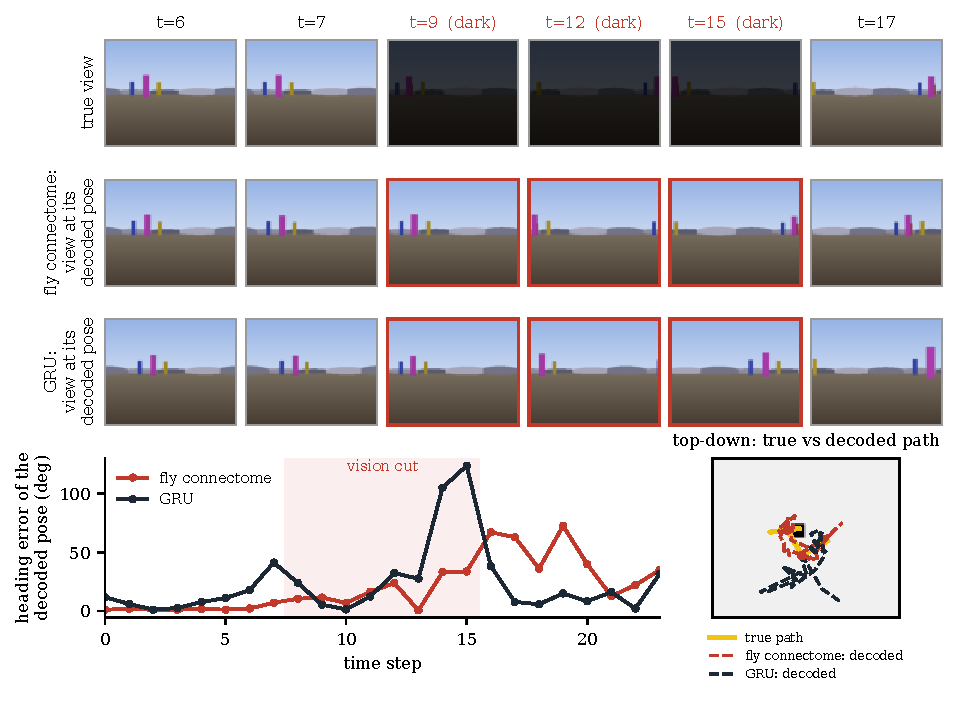
\includegraphics[width=\linewidth]{fig/video_strip.pdf}
  \caption{\textbf{What each network sees, thinks and decodes through a blackout} (one test episode closest to the
  population medians for both models). Top: the panorama the teacher receives, dimmed during the vision cut. Middle: the
  arena rendered at the pose a ridge readout decodes from each student's own activity, so each frame is where the network
  thinks it is. The connectome student's decoded view stays locked to the true view through the dark; the GRU's drifts.
  Bottom: heading error of the decoded pose over time, and the true path against both decoded paths. The readout never
  sees this episode.}
  \label{fig:strip}
\end{figure*}
\begin{table*}[t]
  \centering\small
  \caption{\textbf{Heading and position decoded from the state during 8 dark steps} (ridge probe; median heading
  error in degrees, position $R^2$; mean\pm sd over seeds). The integrator row is the information ceiling; the
  actions-only row is what a linear readout of the action history alone achieves.}
  \label{tab:probe}
  \resizebox{\linewidth}{!}{\begin{tabular}{lcccccc}
    \toprule
    & \multicolumn{2}{c}{Arena} & \multicolumn{2}{c}{Continuous turns} & \multicolumn{2}{c}{NYC twin} \\
    \cmidrule(lr){2-3}\cmidrule(lr){4-5}\cmidrule(lr){6-7}
    wiring & heading err & pos $R^2$ & heading err & pos $R^2$ & heading err & pos $R^2$ \\
    \midrule
    GRU, parameter-matched & 30.6\pm0.6 & 0.41\pm0.01 & -- & -- & 45.4\pm2.6 & 0.25\pm0.01 \\
    GRU, recurrent-budget-matched & 35.5\pm0.7 & 0.30\pm0.01 & -- & -- & -- & -- \\
    dense & 21.3\pm0.7 & 0.68\pm0.01 & -- & -- & -- & -- \\
    connectome, unsigned & 13.8\pm0.8 & 0.88\pm0.01 & -- & -- & -- & -- \\
    connectome, random signs & 9.2\pm1.3 & \textbf{0.94\pm0.01} & -- & -- & -- & -- \\
    \textbf{connectome} & \textbf{9.1\pm1.2} & 0.94\pm0.01 & -- & -- & \textbf{9.4\pm0.7} & \textbf{0.94\pm0.01} \\
    random & 12.9\pm0.7 & 0.88\pm0.01 & -- & -- & 15.1\pm0.7 & 0.89\pm0.00 \\
    block-shuffled & 10.8\pm0.8 & 0.93\pm0.01 & -- & -- & 10.1\pm1.1 & 0.94\pm0.02 \\
    degree-shuffled & 12.7\pm0.6 & 0.89\pm0.02 & -- & -- & 14.3\pm2.0 & 0.84\pm0.01 \\
    \midrule
    actions only (linear floor) & 40.1 & 0.54 & -- & -- & 22.6 & 0.41 \\
    integrator of the action record & 0.0 & 1.00 & -- & -- & 0.0 & 1.00 \\
    \bottomrule
\end{tabular}
}
\end{table*}
\begin{table*}[t]
  \centering\small
  \caption{\textbf{Longer dark windows and a non-linear probe} (arena; heading error, position $R^2$).}
  \label{tab:dark}
  \resizebox{\linewidth}{!}{\begin{tabular}{lcccc}
    \toprule
    wiring & ridge, 8 dark (8:16) & MLP, 8 dark & ridge, 16 dark (8:24) & ridge, 20 dark (4:24) \\
    \midrule
    GRU, parameter-matched & 30.6\pm0.6, 0.41 & 27.4\pm0.3, 0.42 & 37.7\pm0.8, 0.32 & 27.9\pm0.3, 0.50 \\
    GRU, recurrent-budget-matched & 35.5\pm0.7, 0.30 & 32.4\pm0.4, 0.32 & 44.8\pm0.5, 0.21 & 33.7\pm1.0, 0.35 \\
    dense & 21.3\pm0.7, 0.68 & 41.2\pm24.2, 0.27 & 29.9\pm1.1, 0.46 & 21.3\pm0.5, 0.53 \\
    connectome, unsigned & 13.8\pm0.8, 0.88 & -- & -- & -- \\
    connectome, random signs & 9.2\pm1.3, 0.94 & \textbf{4.7\pm0.3, 0.89} & 18.6\pm1.1, 0.82 & 13.6\pm1.4, 0.82 \\
    \textbf{connectome} & \textbf{9.1\pm1.2, 0.94} & 4.7\pm0.1, 0.87 & \textbf{17.7\pm2.1, 0.82} & \textbf{12.6\pm1.2, 0.82} \\
    random & 12.9\pm0.7, 0.88 & 6.4\pm0.4, 0.83 & 24.9\pm0.6, 0.72 & 17.3\pm0.6, 0.77 \\
    block-shuffled & 10.8\pm0.8, 0.93 & 5.9\pm0.3, 0.86 & 23.3\pm0.4, 0.77 & 15.9\pm0.6, 0.77 \\
    degree-shuffled & 12.7\pm0.6, 0.89 & 6.9\pm0.7, 0.83 & 24.0\pm1.0, 0.71 & 17.2\pm0.6, 0.76 \\
    \bottomrule
\end{tabular}
}
\end{table*}
\Cref{tab:probe} is where the wiring pays. The connectome state yields \nConnArenaHd\degree\ median heading error and
position $R^2$ \nConnArenaPos\ on the arena and \nConnNycHd\degree\ / \nConnNycPos\ on NYC; the GRU, which predicts the
latent far better, gives \nGruArenaHd\degree\ / \nGruArenaPos\ and \nGruNycHd\degree\ / \nGruNycPos. Four controls
make the reading safe. (i) The actions-only floor is \nActOnlyArenaHd\degree, so the probe is reading an integral held
by the state, not the raw action input. (ii) A random 762-neuron subset of the connectome (the GRU's width) still beats
the GRU, so feature count is not the explanation (\cref{sec:suppl-probe}). (iii) An MLP probe tightens the connectome
to \nConnArenaMlpHd\degree\ and the GRU only to \nGruArenaMlpHd\degree\ (\cref{tab:dark}), so the GRU's code is not
merely non-linear. (iv) With continuous turn angles the action record no longer determines heading; the continuous-turn probe columns of
\cref{tab:probe} are filled by run 2 (\nSeedsTn\ seeds at the time of writing), and the homing result on that data is
already in \cref{tab:homing}. The code degrades gracefully (\cref{fig:curves}a, \cref{fig:strip}): at 16 dark steps the connectome holds
\nConnArenaDarkSixteenHd\degree\ against \nGruArenaDarkSixteenHd\degree\ for the GRU, and the real wiring's margin over
block-shuffled grows from \nConnBlockGapArena\degree\ to \nConnBlockGapArenaDarkSixteen\degree. Signs matter here where
they did not for prediction: the unsigned graph loses 5\degree. The 51 EPG neurons alone carry almost no heading
($R^2<0.2$); no ring attractor emerges at this scale.

\subsection{Single versus multiple connectomes}
\label{sec:multi}
\begin{figure*}[t]
  \centering
  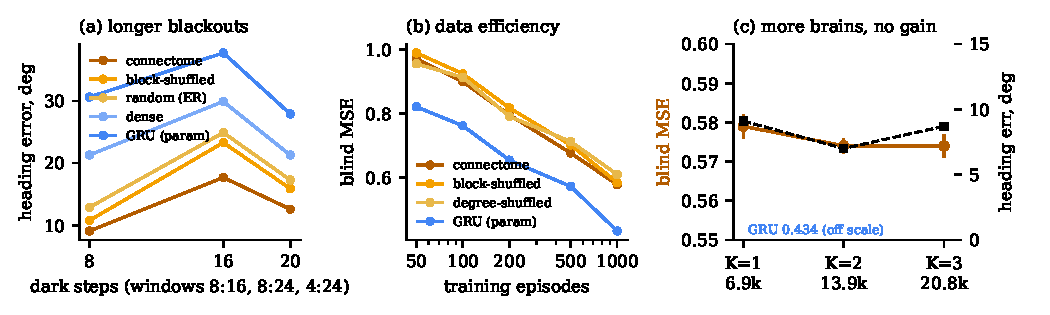
\includegraphics[width=\linewidth]{fig/curves.pdf}
  \caption{\textbf{Robustness of the two findings.} (a) The dark heading code degrades gracefully with the blackout
  length and the sparse-versus-free ordering never changes. (b) From 50 to 1,000 training episodes the GRU leads and the
  connectome beats block-shuffled at every size; a prior that should matter most with little data does not change the
  ranking. (c) Coupling two or three copies of the brain through the real commissural synapses adds neurons but no
  accuracy and leaves the heading code where it was.}
  \label{fig:curves}
\end{figure*}
\begin{table}[t]
  \centering\small
  \caption{\textbf{Multi-brain scaling} (arena, 5 seeds). $K$ copies coupled through the real commissural synapses.}
  \label{tab:multi}
  \begin{tabular}{lcccc}
    \toprule
    $K$ & neurons & synapses & blind MSE & heading err \\
    \midrule
    1 & 6,935 & 91,663 & 0.579\pm0.003 & 9.1\pm1.2 \\
    2 & 13,870 & 183,326 & 0.574\pm0.002 & 7.0 \\
    3 & 20,805 & 274,989 & 0.574\pm0.003 & 8.7 \\
    \bottomrule
  \end{tabular}
\end{table}
Doubling or tripling the brain (\cref{tab:multi}, \cref{fig:curves}c) changes blind MSE by less than one seed standard deviation and
leaves the heading code where it was. The sparse student is therefore not short of neurons or synapses; the gap to
the GRU is a property of the fixed sparse topology, not of its size. One real brain is enough, and we use $K=1$
everywhere else.

\subsection{Sparse state versus dense state: where the gap lives}
\label{sec:gap}
Two thirds of the sparse student's parameters are in the shared linear input map. Replacing it by the cross-attention
encoder, which removes 1.7\,M parameters from every architecture, leaves both the prediction gap and the
path-integration gap in place (\nConnAttnArenaMse\ / \nConnAttnArenaHd\degree\ for the connectome,
\nGruAttnArenaMse\ / \nGruAttnArenaHd\degree\ for the GRU). Adding one attention layer over cell-type tokens to the
connectome recurrence brings MSE to \nHybridArenaMse\ and heading to \nHybridArenaHd\degree. The dense recurrence on
the same neurons predicts better than the connectome (0.562 vs 0.579) but integrates far worse (21\degree\ vs
9\degree), which places it between the two families, exactly where its free weights put it.

\subsection{Benchmark 3: behaviour from the code}
\label{sec:behaviour}
\begin{figure*}[t]
  \centering
  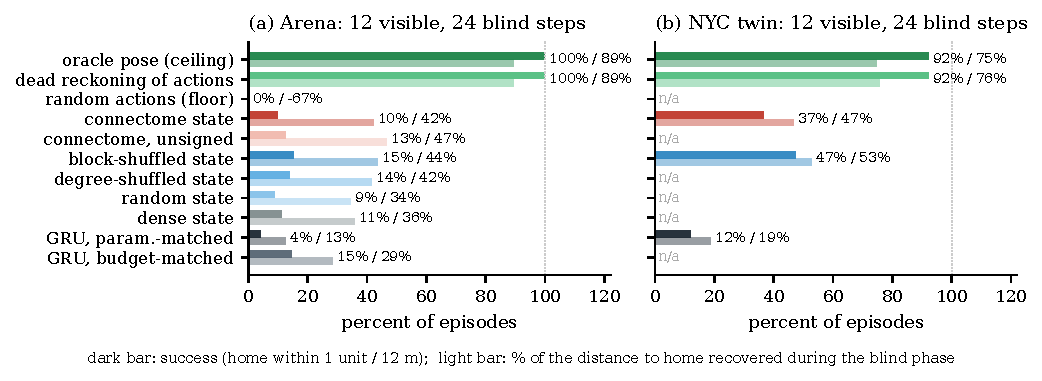
\includegraphics[width=\linewidth]{fig/homing.pdf}
  \caption{\textbf{Blind homing.} After 12 visible steps vision is cut and the same controller steers for 24 steps from
  one of several pose estimates. With the true pose or dead reckoning it gets home almost every time, so the controller
  is not the limit. From a linear readout of a connectome-sized sparse state the agent recovers about half the distance;
  from the GRU state it barely moves. The real wiring has no edge over block-shuffled here.}
  \label{fig:homing}
\end{figure*}
\begin{table*}[t]
  \centering\small
  \caption{\textbf{Blind homing} from a pose decoded linearly from the state (\% of start distance recovered; success
  within 1 unit / 12\,m).}
  \label{tab:homing}
  \resizebox{\linewidth}{!}{\begin{tabular}{lcccccc}
    \toprule
    & \multicolumn{2}{c}{Arena} & \multicolumn{2}{c}{Continuous turns} & \multicolumn{2}{c}{NYC twin} \\
    \cmidrule(lr){2-3}\cmidrule(lr){4-5}\cmidrule(lr){6-7}
    pose readout & \% closer & success & \% closer & success & \% closer & success \\
    \midrule
    oracle pose (controller ceiling) & 89 & 1.00 & -- & -- & 75 & 0.92 \\
    dead reckoning of actions & 89 & 1.00 & 87 & 0.90 & 76 & 0.92 \\
    random actions (floor) & -67 & 0.00 & -- & -- & -- & -- \\
    \midrule
    GRU, parameter-matched state & 13 & 0.04 & 21 & 0.16 & 19 & 0.12 \\
    GRU, recurrent-budget-matched state & 29 & 0.15 & -- & -- & -- & -- \\
    dense state & 36 & 0.11 & -- & -- & -- & -- \\
    connectome, unsigned state & \textbf{47} & 0.13 & -- & -- & -- & -- \\
    \textbf{connectome} state & 42 & 0.10 & \textbf{33} & \textbf{0.16} & 47 & 0.37 \\
    random state & 34 & 0.09 & -- & -- & -- & -- \\
    block-shuffled state & 44 & \textbf{0.15} & -- & -- & \textbf{53} & \textbf{0.47} \\
    degree-shuffled state & 42 & 0.14 & -- & -- & -- & -- \\
    \bottomrule
\end{tabular}
}
\end{table*}
A linear readout of the connectome state drives blind homing to \nConnNycSucc\ success on NYC and \nConnArenaSucc\ on
the arena (\cref{tab:homing}, \cref{fig:homing}), well above the random-action floor and the GRU (\nGruNycSucc, \nGruArenaSucc) but far
below the dead-reckoning ceiling (0.92, 1.00). Block-shuffled homes slightly better than the real wiring. Goal-vector
navigation toward a decoded goal does not beat random actions. The controller is not the bottleneck (the oracle pose
reaches the ceiling); the readout is.

\subsection{Benchmark 4: real handheld video}
\label{sec:realvid}
\begin{figure*}[t]
  \centering
  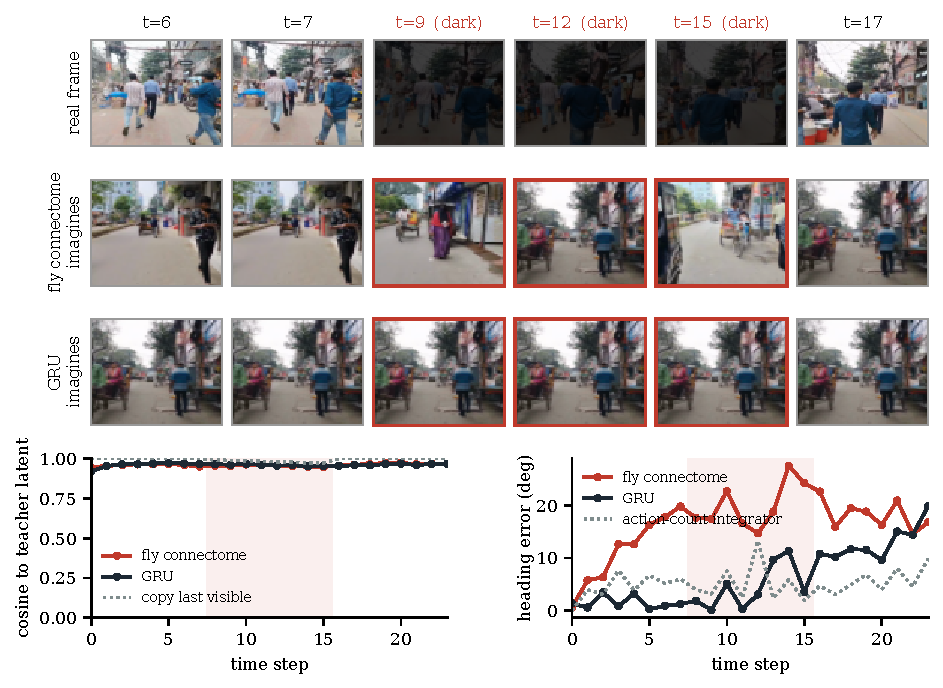
\includegraphics[width=\linewidth]{fig/realvid_strip.pdf}
  \caption{\textbf{The same test on real handheld video} (one held-out phone clip; both students fine-tuned on the other
  clips). Top: the real frame, dimmed during the vision cut. Middle: the training frame whose teacher latent is nearest
  to each student's guess, \ie what each imagines. Bottom left: cosine to the teacher latent against a copy-last
  baseline (dotted). Bottom right: heading decoded from the state against the clip's own egomotion estimate.}
  \label{fig:realvid}
\end{figure*}
\begin{figure}[t]
  \centering
  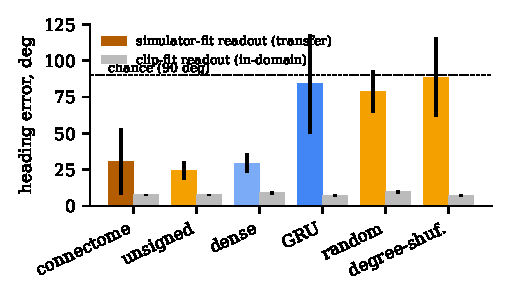
\includegraphics[width=\linewidth]{fig/realvid_bars.pdf}
  \caption{\textbf{Does the heading code transfer from simulator to phone video?} Heading error on real clips with a
  readout fit in the simulator (coloured) or on the other clips (grey). The connectome, unsigned and dense states
  transfer; the GRU, random and degree-shuffled states fall to chance.}
  \label{fig:rvbars}
\end{figure}
\begin{table*}[t]
  \centering\small
  \caption{\textbf{Real phone video} (\nRvClips\ clips, \nRvEpisodes\ episodes): zero-shot and leave-one-clip-out
  fine-tuned MSE, and heading probes with the simulator-fit readout (transfer) or a readout fit on the other clips.}
  \label{tab:realvid}
  \resizebox{\linewidth}{!}{\begin{tabular}{lcccccc}
    \toprule
    wiring & zero-shot MSE & fine-tuned MSE & heading, sim.\ readout & heading, clip readout & NYC model, zero-shot & NYC model, fine-tuned \\
    \midrule
    GRU, parameter-matched & 9.94\pm0.07 & \textbf{1.18\pm0.00} & 84.1\pm34.2 & 7.6\pm0.7 & \textbf{5.57\pm0.03} & -- \\
    dense & 9.73\pm0.07 & 1.21\pm0.04 & 29.5\pm6.4 & 9.1\pm0.9 & -- & -- \\
    connectome, unsigned & 9.59\pm0.13 & 1.26\pm0.00 & \textbf{24.3\pm6.3} & 7.7\pm0.3 & -- & -- \\
    \textbf{connectome} & 9.68\pm0.10 & 1.24\pm0.02 & 30.9\pm22.8 & 7.7\pm0.5 & 6.10\pm0.03 & -- \\
    random & \textbf{9.56\pm0.19} & 1.26\pm0.01 & 79.1\pm14.5 & 9.9\pm1.1 & 6.00\pm0.02 & -- \\
    degree-shuffled & 9.69\pm0.09 & 1.25\pm0.02 & 88.7\pm27.0 & \textbf{7.1\pm0.6} & 6.01\pm0.05 & -- \\
    \midrule
    copy last visible latent & 0.84 & 0.84 & -- & -- & 0.84 & 0.84 \\
    constant mean & 10.28 & 10.28 & -- & -- & 10.28 & 10.28 \\
    actions only (linear floor) & -- & -- & -- & 4.7 & -- & -- \\
    \bottomrule
\end{tabular}
}
\end{table*}
Zero-shot, no student beats the copy-last predictor on real footage (\cref{tab:realvid}): the simulator-to-phone gap
swamps every architectural difference. After fine-tuning all students land within 7\,\% of each other. The heading
probe is the informative row (\cref{fig:rvbars}): with the \emph{simulator-fit} readout the connectome and unsigned connectome transfer at
\nConnArenaRvTransferHd\degree\ and \nNosignArenaRvTransferHd\degree\ while the GRU, random and degree-shuffled states
do not transfer at all (79 to 89\degree); with an in-domain readout every state decodes heading to 7 to 10\degree.

\subsection{What is outperformed, and what is not}
\label{sec:scorecard}
\begin{table}[t]
  \centering\footnotesize
  \caption{\textbf{Scorecard.} Does the connectome beat each baseline on each benchmark? \checkmark\ yes (5 seeds,
  paired $p<0.01$); $\approx$ within seed noise; $\times$ no.}
  \label{tab:score}
  \setlength{\tabcolsep}{3pt}\begin{tabular}{lcccc}
    \toprule
    baseline & MSE & heading & homing & real-video \\
    \midrule
    degree-shuffled & \checkmark & \checkmark & $\approx$ & \checkmark \\
    random (ER) & \checkmark & \checkmark & \checkmark & \checkmark \\
    block-shuffled & \checkmark & \checkmark & $\times$ & -- \\
    random signs & $\approx$ & $\approx$ & -- & -- \\
    unsigned & $\times$ & \checkmark & $\times$ & $\approx$ \\
    dense & $\times$ & \checkmark & \checkmark & $\approx$ \\
    GRU (param-matched) & $\times$ & \checkmark & \checkmark & \checkmark \\
    GRU (recurrent-matched) & $\times$ & \checkmark & \checkmark & -- \\
    transformer & $\times$ & \checkmark & -- & -- \\
    \bottomrule
  \end{tabular}
\end{table}
\Cref{tab:score} condenses the paper. The connectome beats every \emph{wiring} control on prediction and on the dark
heading code. It loses prediction to every \emph{free} recurrence and wins the dark heading code against all of them.

\subsection{Cost, scaling and ablation}
\label{sec:more}
One connectome step costs 7.4\,MFLOP, the same as the parameter-matched GRU, with 91,663 recurrent weights against
the GRU's 580,644; dense costs 103\,MFLOP. With the synapse threshold at 1, 5 or 10, with MB or OUT removed, or with CX
alone, the real wiring beats its degree-shuffled twin by 0.02 to 0.04 MSE (\cref{sec:ablation}); no single region
carries the margin.
